\chapter{X joslas raidīšanas sistēmas vadības bloka prototipa izstrāde}

Šajā nodaļā ir izklāstīta šī bakalaura darba ietvaros veiktā X joslas raidīšanas sistēmas vadības bloka prototipa izstrāde. Sākas nodaļa ar sistēmas pārskatu, tad tiek aprakstīts darba punkta iestatīšanas izstrādes process, kur tiek aprakstītas izveidotās iespiedplates, pēc kā tiek pievērsta uzmanība mikrokontrolierim, programmas kodam un lietojumprogrammas izstrādei, tad tiek aprakstīta jaudas monitorēšanas sistēmas izstrāde, kur beigās ir gala prototipu apraksts, kur tiek aprakstīts atsevišķo sistēmu novietojums korpusā. Visas izstrādnes, kas tika izstrādātas šī bakalaura ietvaros, tiek uzglabātas githubā\cite{bak_github}.

\section{RT-16 X-joslas raiduztverošās sistēmas pārskats}
Att 1.1. tiek parādīta X-joslas pārskats RT-16 radioteleskopam. Sistēmas vadība tiek veikta ar operatora jeb kontroles datoru, kas vada Cortex modemu \cite{cortex}, frekvenču lejuppārveidotāju un augšuppārveidotāju \cite{up_down_converters}, LNA un HPA. Cortex modēms paredzēts datu modulēšanai un demodulēšanai no satelīta. Frekvenču lejup un augšup pārveidotājs nepieciešams, lai varētu modulēto signālu pārnest uz nepieciešamo nesējfrekvenci noteiktam satelītam. HPA pastiprina modulēto signālu līdz 100 W (+50 dBm), lai palielinātu pārraides attālumu. HPA bloka pārraides jaudu noteica SSC. LNA nepieciešams, lai uzlabotu uztvertā signāla SNR un lai Cortex varētu to veiksmīgi demodulēt. Dipleksers un paraboliskā antena paredzēti signāla uztveršanai un pilna dupleksa komunikācijas nodrošināšanai.
\begin{figure}[H]
	\centering
    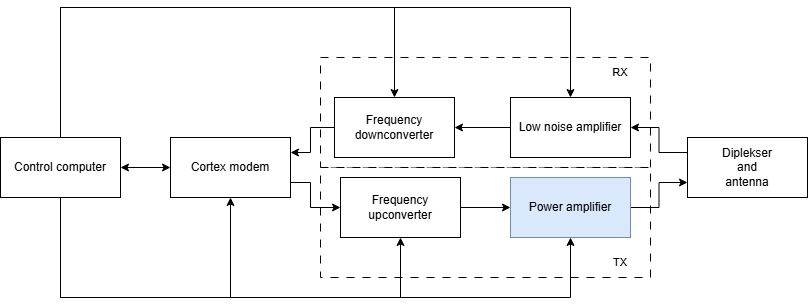
\includegraphics[width=\textwidth]{pictures/rt-16_x_diagram.jpg}\hspace{1cm}
    \caption{RT-16 X-joslas raiduztvērēja vispārīga bloka diagramma}
\end{figure}
Turpmāk darbā tiek apskatīts tikai augstas jaudas pastiprinātājs, kur daļa no tā tiek izstrādāta šī bakalaura ietvaros.
\section{Darba punkta nodrošināšanas sistēmas izstrāde}
Šajā nodaļā tiek aprakstīta izstrādes plates modifikācija un testēšana, izstrādātie līdzstrāvas sprieguma pārveidotāji, industriālā barošanas avota vadības, strāvas mērīšanas, ieslēgšanas/izslēgšanas elektriskā principiālā shēmas. Daļas, kas nodrošina darba punkta iestatīšanas/atiestatīšanas funkciju.
\subsection{Monitoringa izstrādes plates modifikācija un integrēšana}
Lai ātrāk iegūtu vēlamo rezultātu, tika iegādāta izstrādes plate ar izvēlēto monitorēšanas integrālo shēmu EVAL-AD7293 \cite{eval_board} ar AD piedāvātu vadības sistēmu EVAL-SDP-CB1Z \cite{eval_board_mcu}.
\begin{figure}[H]
	\centering
    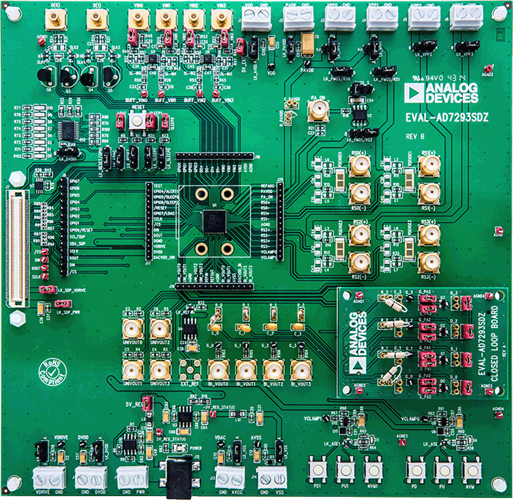
\includegraphics[width=0.5\textwidth]{pictures/EVAL-AD7293SDZ_TOP-web.png}\hspace{1cm}
    \caption{AD7293 izstrādes plate}
\end{figure}
\begin{figure}[H]
	\centering
    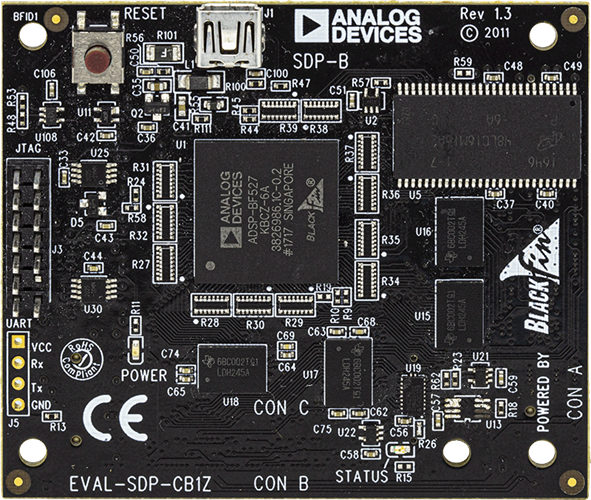
\includegraphics[width=0.5\textwidth]{pictures/EVAL-SDP-B-top-web.png}\hspace{1cm}
    \caption{Vadības sistēma monitorēšanas izstrādes platei}
\end{figure}
Šīs sistēmas pārbaudei tika izmantota AD lietojumprogramma, kas sniedz vispārīgu pārskatu par sistēmas funkcionalitāti.
\begin{figure}[H]
	\centering
    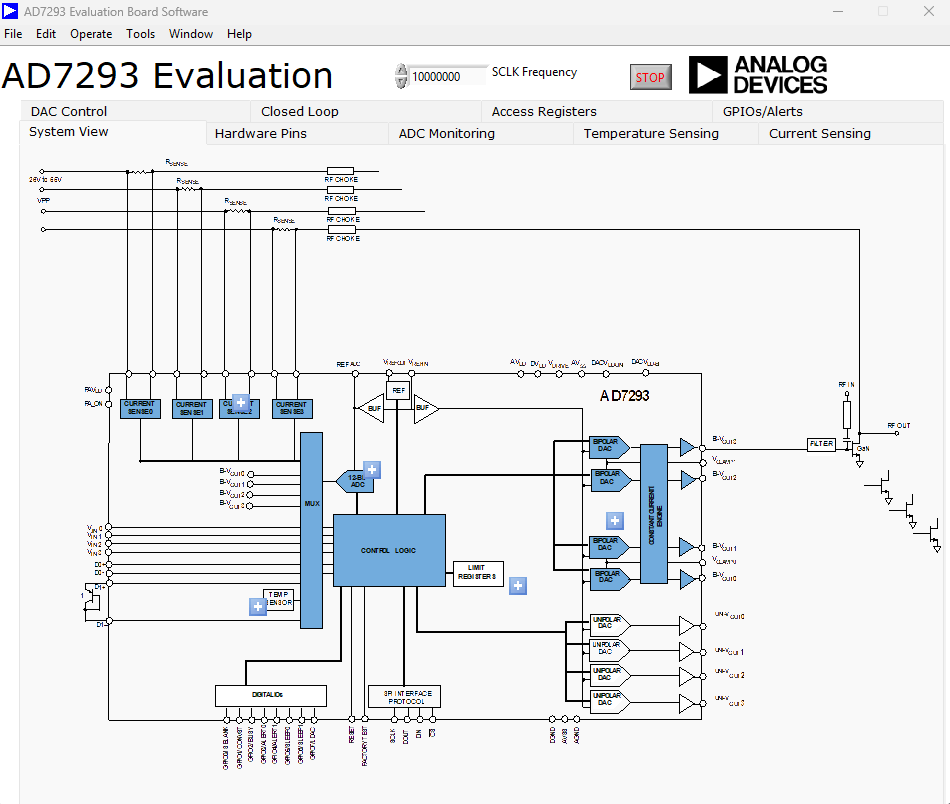
\includegraphics[width=0.6\textwidth]{pictures/eval-soft.png}\hspace{1cm}
    \caption{AD7293 testēšanas lietojumprogramma}
\end{figure}
Sekojot datu lapā pieejamai informācijai tika nodrošināta reģistru konfigurācijas secība un sasniegta vēlamā funkcionalitāte darba punkta iestatīšanai un atiestatīšanai.\\
Pēc nepieciešamās funkcionalitātes nodrošināšanas tika veiktas izstrādes plates modifikācijas - atlodēti SMA konektori, lai varētu pielodēt strāvas monitorēšanas sistēmas izvadus un ieslēgšanas/izslēgšanas sistēmas vadības izvadu, samainīti savienotājelementi, pievienoti barošanas avoti un pievienots digitālās loģikas analizators, lai monitorētu SPI saskarni.
\begin{figure}[H]
	\centering
    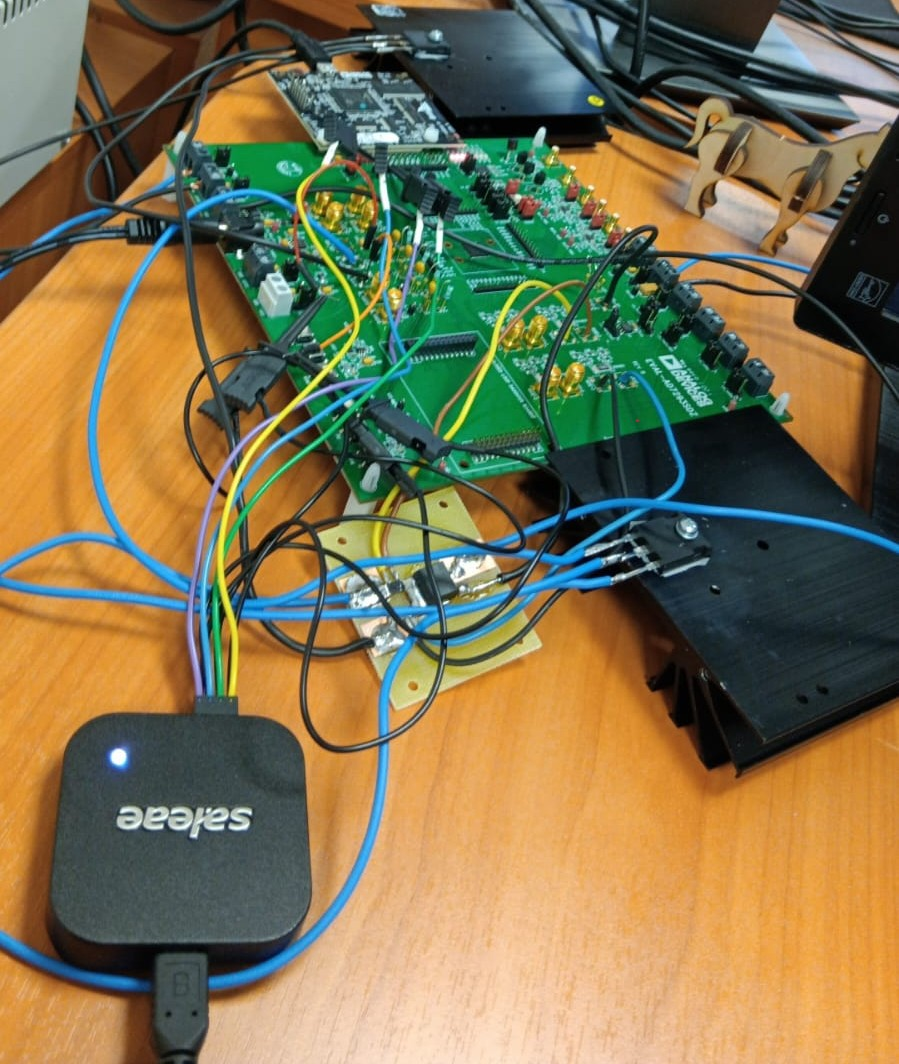
\includegraphics[width=0.5\textwidth]{pictures/daf.jpg}\hspace{1cm}
    \caption{Testa stends ar testa lauktranzistoriem}
\end{figure}
Tad tika sasniegts vēlamais rezultāts ar darba punkta iestatīšanu un atiestatīšanu.
\subsection{Sprieguma pārveidotāji, temperatūras sensora un 24 V barošanas avota vadības shēmas}
Tika izvēlēti lineārie sprieguma stabilizatori 5 un 9 V līnijām, neskatoties uz zemo efektivitāti, salīdzinot ar impulsa tipa sprieguma stabilizatoriem, tie nerada trokšņus izejā. Lineārie sprieguma stabilizatori tiek slēgti virknē, lai palielinātu 5 V regulātora efektivitāti, samazinot sprieguma kritumu uz tā. 12 V tiek pārveidots uz 9 V un no 9 V tiek pārveidots uz 5 V.  
\begin{figure}[H]
	\centering
    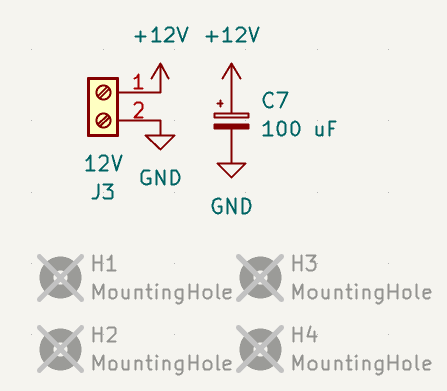
\includegraphics[width=0.6\textwidth]{pictures/inputs.png}\hspace{1cm}
    \caption{Ievadi, elektrolītiskais kondesators un urbjcaurumi}
\end{figure}
J3 terminālbloks ir paredzēts, lai varētu pieslēgt industriālo 12 V barošanas avotu. C7 elektrolītiskais kondensators paredzēts, lai mazinātu ieejas pulsācijas. H1, H2, H3 un H4 urbjcaurumi paredzēti, lai iespiedplati varētu iestiprināt korpusā.
\begin{figure}[H]
	\centering
    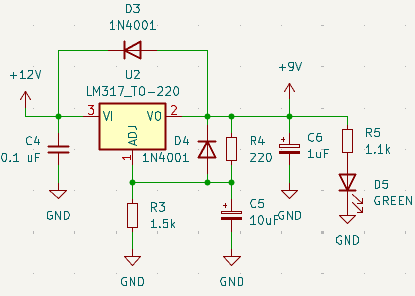
\includegraphics[width=0.6\textwidth]{pictures/9v.png}\hspace{1cm}
    \caption{12 V uz 9 V pārveidotais}
\end{figure}
\begin{figure}[H]
	\centering
    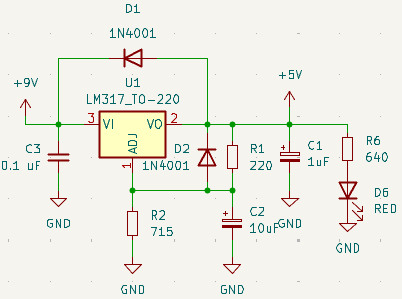
\includegraphics[width=0.6\textwidth]{pictures/5v.png}\hspace{1cm}
    \caption{9 V uz 5 V pārveidotais}
\end{figure}
Sprieguma iestatīšanai tiek izmantota atgriezeniskā saite, ko veido rezistori R1, R2, R3 un R4. Ķēdē tiek izmantoti keramiskie kondensatori C1, C3, C4 un C6. keramiskie un elektrolītiskie kondensatori ir vajadzīgi, lai mazinātu barošanas pulsācijas. R6 un R5 ir strāvas ierobežojošie rezistori D5 un D6 gaismas diodēm. D1, D2, D3 un D4 taisngriežu diodes paredzētas, lai neļautu C2 un C5 kondensatoriem izlādēties lineārā sprieguma izejā.
\begin{figure}[H]
	\centering
    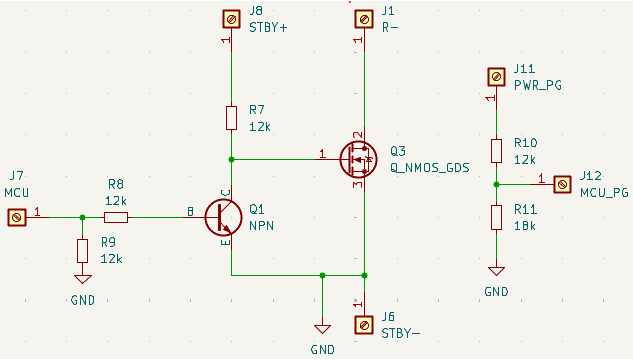
\includegraphics[width=0.6\textwidth]{pictures/24_control_detection.png}\hspace{1cm}
    \caption{24 V barošanas avota vadības sistēmu}
\end{figure}
J7 izvads paredzēts, lai varētu pieslēgt mikrokontrolliera vadības signālu. R8 ir paredzēts strāvas ierobežošanai NPN bipolārajam tranzistoram. R9 ir zema līmeņa piesaistes rezistors, lai pārejas procesā netiktu atvērts tranzistors. R7 rezistors ir paredzēts strāvas ierobežošanai un augsta signāla līmeņa piesaistei pie N kanāla lauktranzistora aizvara. J8, J1 un J6 izvadi paredzēti, lai varētu vadīt 24 V industriālo barošanas avotu. J11 ir paredzēts barošanas avota stāvokļa pieslēgvieta, kur R10 un R11 rezistori ir sprieguma dalītāji, lai varētu veikt sprieguma nolasi ar mikrokontrolliera.
\begin{figure}[H]
	\centering
    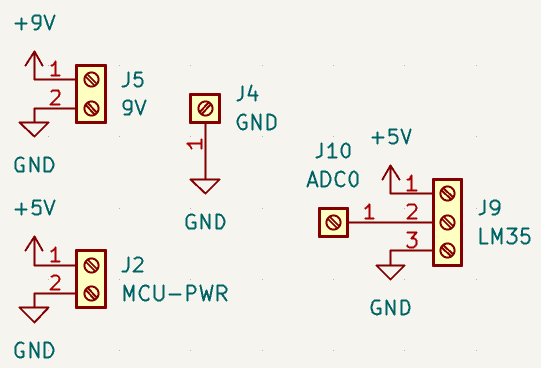
\includegraphics[width=0.6\textwidth]{pictures/outputs.png}\hspace{1cm}
    \caption{Pieslēgvietas MCU, temperatūras un patērētājiem}
\end{figure}
J5 un J2 terminālbloks paredzēts, lai varētu nodrošināt 9 V un 5 V barošanu patērētājiem. J9 terminālbloks paredzēts temperatūras sensora pieslēgšanai. J10 ir izvads, paredzēts mikrokontroliera ADC pieslēgvietai.
\begin{figure}[H]
	\centering
    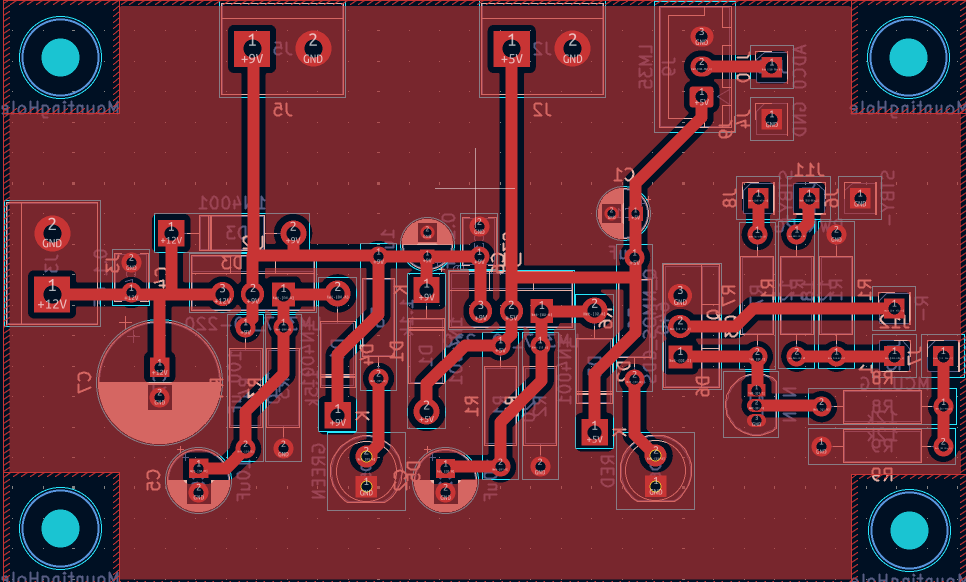
\includegraphics[width=0.6\textwidth]{pictures/power_board.png}\hspace{1cm}
    \caption{Iespiedplate lietojumprogrammatūrā "KiCad"}
\end{figure}
 Iespiedplate tika trasēta vienā slānī. Komponentes tika izvietotas pēc iespējas blīvāk, lai samazinātu iespiedplates izmērus. Tika izmantotas THT komponentes. Iespiedplate tika izfrēzēta ar augstskolā pieejamo frēzi.
\subsection{Strāvas mērīšanas iespiedplate ar ieslēgšanas/izslēgšanas slēdzi}
\begin{figure}[H]
	\centering
    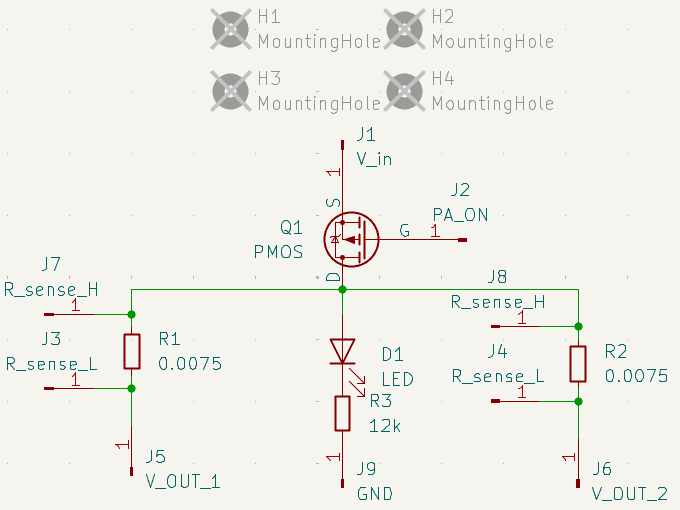
\includegraphics[width=0.6\textwidth]{pictures/shunt_resistors.png}\hspace{1cm}
    \caption{Strāvas mērīšanas shematiskais zīmējums}
\end{figure}
J1 terminālbloks ir 24 V pieslēgvietas nodrošināšanai. Q1 P kanāla lauktranzistors tiek izmantots slēdža režīmā, kas tiek kontrolēts ar AD7293 monitorēšanas integrālo shēmu, kas tiek pievadīts caur J2 termināli. R1 un R2 ir šunta rezistori strāvas mērīšanai. Šunta rezistori tika aprēķināti pēc izvēlētā mērīšanas diapazona AD7293 un maksimālās strāvas R <= 0.025/3 . J3, J4, J7 un J8 izvadi ir paredzēti, lai pieslēgtu strāvas mērīšanas sistēmu. D1 gaismas diodē ir paredzēta sistēmas stāvokļa identificēšanai. R3 rezistors ir paredzēts strāvas ierobežošanai, lai pasargātu gaismas diodi. J9 izvads paredzēts zemējuma nodrošināšanai.
\begin{figure}[H]
	\centering
    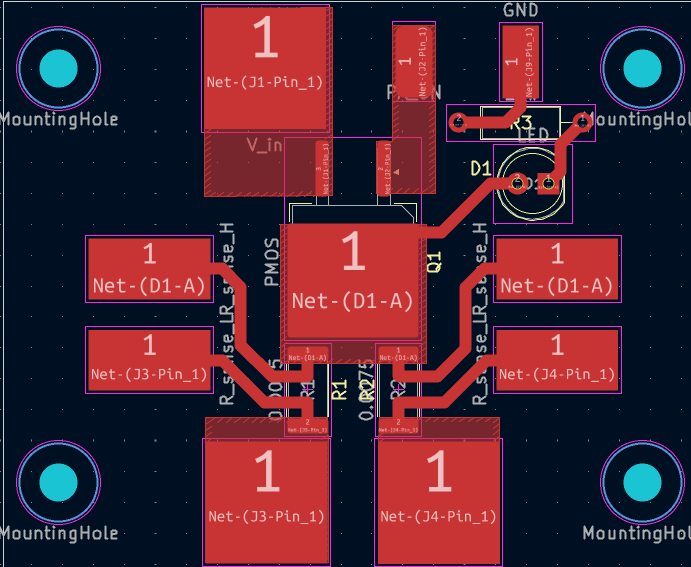
\includegraphics[width=0.6\textwidth]{pictures/shunt_resistors_board.png}\hspace{1cm}
    \caption{Iespiedplate lietojumprogrammatūrā "KiCad"}
\end{figure}
Tika izstrādāta vienslāņu plate ar blīvu komponenšu izvietojumu un attiecīgu jaudas celiņu platumiem. Tā tika izfrēzēta ar VeA pieejamo frēzi.

\section{Mikrokontroliers un vadības sistēma caur tīklu}
Kā mikrokontrolieris tika izvēlēts W5500-EVB-Pico \cite{pico}, balstoties uz darba vadītāja ieteikumu, kam ir TCP/IP tīkla steka atbalsts, ar kuru ir gatavi TCP servera piemēri, kas saņem un nosūta komandas tīklā, kā arī mikrokontrolierim ir divi kodoli.
\begin{figure}[H]
	\centering
    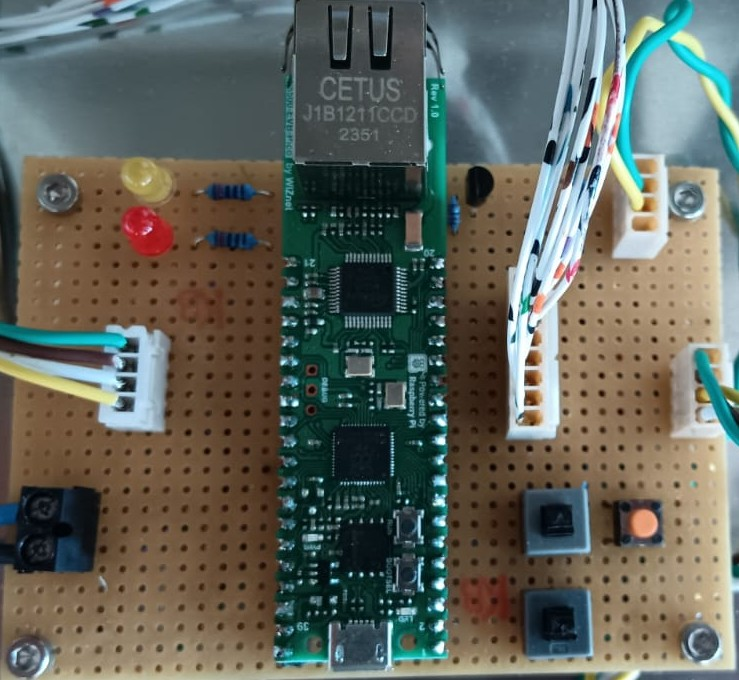
\includegraphics[width=0.6\textwidth]{pictures/mcu_board.jpg}\hspace{1cm}
    \caption{Mikrokontroliera iespiedplate}
\end{figure}
RP4020 mikrokontrolieris tiek plaši pielietots iegultajās sistēmās, jo viena mikroshēma satur CPU, atmiņu, RAM, watchdogs u.c. perifērijas. Tika izvēlēts Arduino IDE šim mikrokontrolierim, izmantojot C un C++ programmēšanas valodas. Arduino vide tika izvēlēta dēļ gatavo bibliotēku pieejamības WS5500 tīkla modulim \cite{ws5500}, un VSRC izstrāde ir balstīta uz šīm bibliotēkām.
\begin{figure}[H]
	\centering
    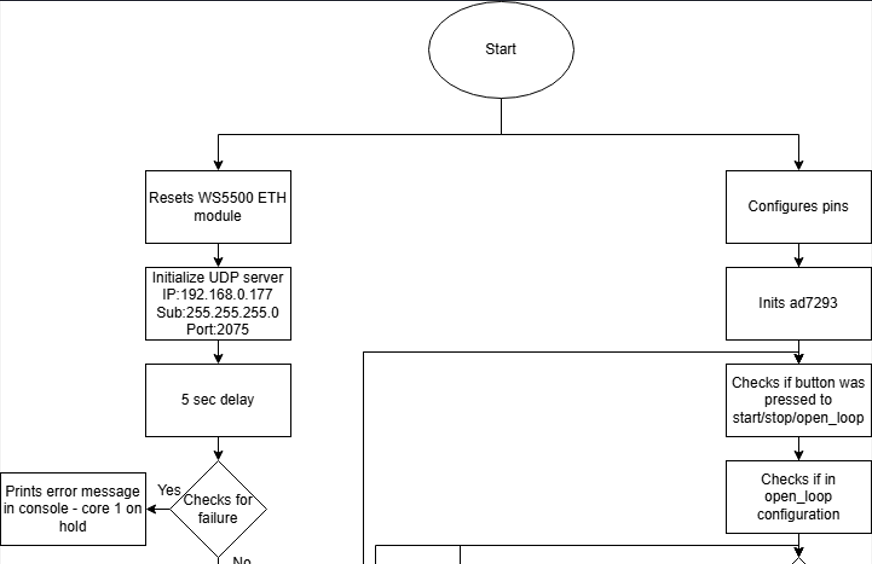
\includegraphics[width=0.8\textwidth]{pictures/prog_code_1.png}\hspace{1cm}
    \caption{Daļa no programmas koda bloka diagramma}
\end{figure}
Divkodolu mikrokontrolierim tiek izmantots viens kodols servera uzturēšanai un datu pārraidei, bet otrā tiek kontrolēti mikrokontroliera izvadi, monitorēšanas integrālā shēma, temperatūras mērīšana un sistēmas statusa noteikšana. Programmas kods sākas ar to, ka pirmajā kodolā tiek restartēts un konfigurēts WS5500 modulis, tad tiek konfigurēts izvadīts kļūdas paziņojums, tas tiek darīts 3 reizes un pēc trešās reizes, ja nesanāk, tad kodols tiek apstādināts. Otrā kodolā nokonfigurē izvadus un darba punkta un monitorēšanas integrālo shēmu. Tad tiek pārbaudīts, vai ir nospiesta viena no trim pogām. Spiedpogas paredzētas manuālai testēšanai, kur pirmā spiedpoga atbild par sistēmas ieslēgšanu un darba punkta nodrošināšanu, otrā spiedpoga nodrošina sistēmas izslēgšanu un darba punkta atiestatīšanu, bet trešā, lai deaktivizētu slēgto ciklu, lai varētu pārraidīt RF signālu ar mainīgu jaudu. Tiek pārbaudīts, vai ir atvērtā cikla konfigurācijā, ja jā, tad tiek aktivizēta gaismas diode, kas atrodas uz mikrokontroliera plates.
\begin{figure}[H]
	\centering
    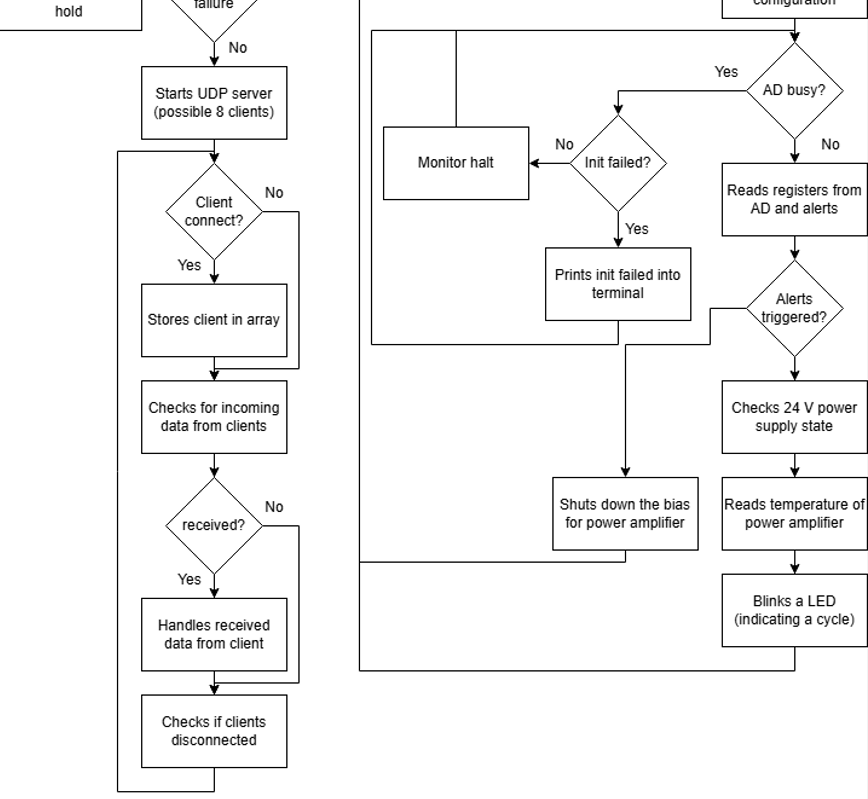
\includegraphics[width=0.8\textwidth]{pictures/prog_code_2.png}\hspace{1cm}
    \caption{Daļa no programmas koda bloka diagramma}
\end{figure}
Pirmajā kodolā tiek uzsākts serveris, pie kura var pieslēgties līdz astoņiem klientiem. Pirmajā kodolā tiek pārbaudīts, vai ir jauns klienta pieslēgšanās pieprasījums, ja ir, tad klienta TCP objektu saglabā masīvā, kas glabā informāciju par klienta IP adresi un portu, kā arī savienojuma stāvokli, bet, ja nav, tad pārbauda, vai ir saņemti komandas no klientiem, ja tādi ir, ja kādi dati ir saņemti, tad to apstrādā un veic attiecīgu darbību, bet, ja nav, tad pārbauda, vai kāds klients ir atslēdzies no servera, lai varētu atbrīvot masīvu un vietu citam klientam. Otrā kodolā tiek pārbaudīts, vai monitorēšanas integrālā shēma ir aizņemta, tas datu lapā netiek uzsvērts, bet pārbaude netraucē, ja ir, tad pārbauda, vai tā tiek izmantota citā procesā vai ir inicializācijas problēmas, tad pārbauda tās statusu atkal. Ja AD7293 ir gatavs komunikācijai, tad tiek nolasīti reģistri un karodziņi, ja kāds no karodziņiem tiek aktivizēts, tad darba punktu atiestata un atslēdz sistēmu, bet, ja nav, tad tiek pārbaudīts 24 V elektrobarošanas statuss, nolasīta temperatūra un ieslēdz un ar aizskavi izslēdz gaismas diodi, kas atspoguļo viena cikla beigas.\\
Mikrokontrolieris saglabā sistēmas esošo stāvokli mainīgajā, nolasa datus no sensoriem un monitorēšanas integrālās shēmas datus, kuri tiek strukturizēti simbolu virknē un nosūtīti caur TCP protokolu klientam pēc pieprasījuma. Zemāk apkopota telemetrijas virkne.
\begin{table}[H]
\centering
\captionsetup{singlelinecheck=off, justification=raggedleft}
\caption{Telemetrijas virknes struktūra un atšifrējums}
\renewcommand{\arraystretch}{1.2}
\begin{tabular}{|c|c|l|l|}
\hline
\multirow{24}{*}{\centering 96 baiti} & \textbf{Datu tips} & \textbf{Mainīgā nosaukums} & \textbf{Definīcija} \\
\hline
\cline{2-4}
& I    & pa\_on\_state          & HPA stāvoklis (0=off, 1=on) \\
\cline{2-4}
& I    & psu\_pg\_state         & Barošanas avota status (0=off, 1=on) \\
\cline{2-4}
& I    & open\_loop\_mode       & Kontroles režīms (0=closed, 1=open) \\
\cline{2-4}
& F    & rs0\_volts            & Noteces spriegums HPA \\
\cline{2-4}
& UI   & rs\_alert\_high       & Maksimālā noteces slieksņa brīdinājums\\
\cline{2-4}
& UI   & rs\_alert\_low        & Minimālā noteces slieksņa brīdinājums\\
\cline{2-4}
& UI   & alert0\_state         & Sistēmas brīdinājumu status \\
\cline{2-4}
& F    & isense0\_amps         & Strāvas mērījums 0 kanālam\\
\cline{2-4}
& F    & isense1\_amps         & Strāvas mērījums 1 kanālam\\
\cline{2-4}
& F    & Ug0\_volts            & Aizvara sprieguma 0 mērījums \\
\cline{2-4}
& F    & Ug0\_volts\_lim       & Aizvara sprieguma 0 limits \\
\cline{2-4}
& F    & Ug1\_volts            & Aizvara sprieguma 1 mērījums \\
\cline{2-4}
& F    & Ug1\_volts\_lim       & Aizvara sprieguma 1 limits \\
\cline{2-4}
& F    & temp\_degC            & Temperatūra korpusā \\
\cline{2-4}
& F    & temp1\_degC           & Temperatūra uz HPA 1 \\
\cline{2-4}
& F    & temp2\_degC           & Temperatūra uz HPA 2 \\
\cline{2-4}
& F    & temp\_degC\_Fpwr      & Izstarotā jaudas mērītāja temperatūra \\
\cline{2-4}
& F    & temp\_degC\_Rpwr      & Atstarotās jaudas mērītāja temperatūra\\
\cline{2-4}
& F    & temp\_degC\_AD7293      & Monitorēšanas IC temperatūra\\
\cline{2-4}
& F    & reflected\_power\_log      & Atstarotā jauda dBm \\
\cline{2-4}
& F    & reflected\_power\      & Atstarotā jauda W\\
\cline{2-4}
& F    & forward\_power\_log        & Izstarotā jaudas dBm \\
\cline{2-4}
& F    & forward\_power\        & Izstarotā jaudas W \\
\cline{2-4}
& F    & $S_{11}$\_param\        & Izstarotā jaudas W \\
\hline
\end{tabular}
\end{table}
 Struktūra sastāv no 96 baitiem. Pirmie 4 baiti satur esošo jaudas pastiprinātāja stāvokli (izslēgts, ieslēgts), otrie 4 baiti satur 24 V elektrobarošanas statusu (ieslēgts, izslēgts), trešie 4 baiti satur informāciju par to, vai ir cikla konfigurācijā, ceturtie 4 baiti, kas atgriež sprieguma kritumu uz šunta rezistora, tad nākošie 4 baiti atgriež karodziņu vecāko un jaunāko baitu, tad nākošie četri ir karodziņi. Isens0 atgriež strāvas vērtību caur pirmo šunta rezistoru, kur Isense1 atgriež strāvas vērtību caur otro šunta rezistoru. Tālāk iet UG0 volti, kas nosaka, kāds ir aizvara vadības sprieguma līmenis pirmajam pastiprinātājam, tad ir ierobežojums, kas nosaka iestatītās robežvērtības, tad nākošie 8 baiti nozīme ir ekvivalenta tikai otram pastiprinātājam. Nākošie 4 baiti ir temperatūras mērījums korpusā, tad 8 baiti ir temperatūras mērījumi divos punktos uz jaudas pastiprinātāja, tad nākošie 8 baiti ir jaudas mērītāju IC temperatūra izstarotajai un atstarotajai jaudai un 4 baiti monitorēšanas IC temperatūra. Nākošie 16 baiti ir izstarotās un atstarotās jaudas logaritmiskā un matemātiskā reprezentācijā. Pēdējais ir S11 parametrs.\\
 Klients var nosūtīt vairākas komandas mikrokontrolierim, lai iestatītu režīmu, mainītu konfigurāciju un pieprasītu datus.
 \begin{table}[H]
\centering
\captionsetup{singlelinecheck=off, justification=raggedleft}
\caption{Iespējamās komandas un to atšifrējums}
\renewcommand{\arraystretch}{1.2}
\begin{tabular}{|c|c|l|l|}
\hline
\multirow{6}{*}{\centering 15 baiti} & \textbf{Datu tips} & \textbf{Mainīgā nosaukums} & \textbf{Definīcija} \\
\hline
\cline{2-4}
& S    & mon          & Pieprasa telemetrijas virkni \\
\cline{2-4}
& S    & pon          & Aktivizē/deaktivizē sistēmu \\
\cline{2-4}
& S    & olm          & Maina noslēgtās cilpas konfigurāciju \\
\cline{2-4}
& S    & setcurr          & Iestata noteces strāvu kanāliem \\
\cline{2-4}
& S    & setramp          & Iestata darba punkta iestatīšanas periodu \\
\hline
\end{tabular}
\end{table}
Maksimālā simbola virkne, ko var apstrādāt mikrokontrolieris, ir 15 baiti. Mon komanda ir vienīgā, kura nepieņem papildus argumentus, mikrokontrolieris saņemot šo komandu, atbild nekavējoties ar telemetrijas virkni klientam. Pon komanda pieņem vienu argumentu 0 vai 1, ja tiek saņemts 1, tad tiek uzsākta sistēmas darbība (elektrobarošanas ieslēgšana, darba punkta nodrošināšana u.c.), bet, ja saņem 0, tad sistēmas darbība tiek pārtraukta (darba punkta atiestatīšana, elektrobarošanas izslēgšana u.c.). Olm komanda pieņem vienu argumentu 0 vai 1, ja saņemts ir 1, tad slēgtais cikls tiek izslēgts, ja saņem 0, tad to aktivizē. Ja tiek padoti nepareizi ieejas argumenti, tad sistēma atbild ar iespējamajiem variantiem lietotājam. Setcurr komanda pieņem peldošā komata mainīgo, kas iestata darba punkta strāvu visiem kanāliem. Setramp pieņem float argumentu, ar kuru var izmainīt darba punkta noturēšanas strāvu no 250~\textmu s līdz 31.75~ms
\begin{figure}[H]
	\centering
    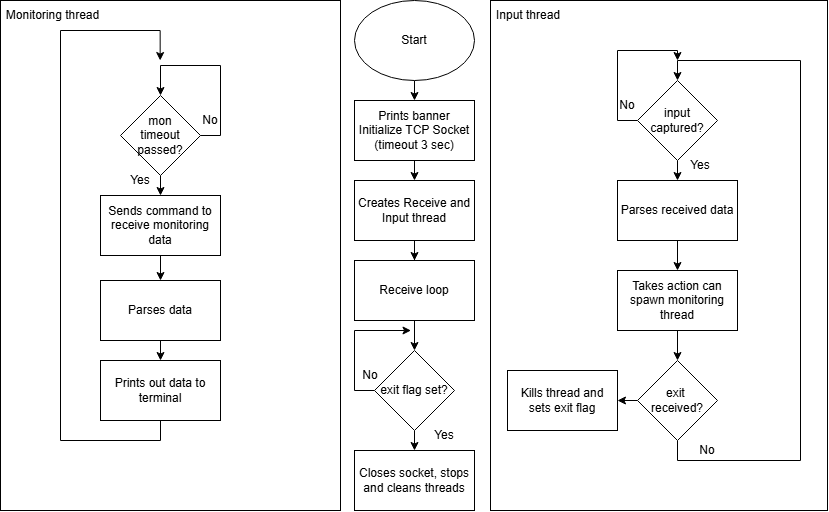
\includegraphics[width=0.8\textwidth]{pictures/script_program.drawio.png}\hspace{1cm}
    \caption{Python skripta bloka diagramma}
\end{figure}
Tika izveidots Python skripts uz Windows 11 OS, kas uzsāk X-joslas sistēmas darbību. Skriptu startējot, tiek terminālī izvadīts logo, atšifrējums, sistēmas nosaukums un palīginstrukcija ar visām iespējamām darbībām. Tad tiek izveidots TCP klients, kurš mēģina pieslēgties pie TCP servera ar 3 sekunžu intervālu; ja neizdodas, skripts beidz savu darbu. Kad ir izveidots savienojums ar serveri, tad skripts izveido ievades pavedienu un ieiet uztveršanas ciklā. Uztveršanas cikls gaida ienākošo simbolu virkni un saņemšanas brīdī to izvada; ja nekas netiek saņemts, tad tiek izvadīts paziņojums, ka serveris ir pārtraucis kontaktēties, un beidzas skripta darbība. Ievades pavedienā tiek termināli izvadīts teksts ar aicinājumu uzsākt sistēmas darbību ar "start", kas uzsāk X-joslas sistēmas darbību, aktivizējot sistēmu un iestatot darba punktu ar noklusējuma vērtībām. Kad tiek saņemta simbolu virkne, tā tiek pārbaudīta, vai virkne atbilst kādai no iespējamajām funkcijām; ja nē, tas tiek automātiski nosūtīts mikrokontrolierim. Ja komanda atbilst kādai no skripta funkcionalitātēm, tad tā tiek parsēta un attiecīgi izvadīta informācija vai pārtraukta tās darbība. Kad tiek nosūtīta start komanda, skripts izveido monitorēšanas pavedienu, kur ik pēc iestatītā intervāla tiek veikta telemetrijas virknes nolase no mikrokontroliera, tad ienākošā telemetrija tiek parsēta un izvadīta lietotājam ērtākā virtenē. Ja tiek saņemta "exit" komanda vai ctrl+c kombinācija, tad automātiski sistēma pārtrauc savu darbību un pārbauda, vai kāds no pavedieniem ir aktīvs; ja ir, tad to pārtrauc, kā arī tiek pārbaudīts sistēmas stāvoklis; ja tas ir ieslēgts, tad to izslēdz pirms skripts aizveras.
\section{Jaudas detektora izstrāde}
Ir divas jaudas mērīšanas integrālās shēmas, kas veic atstarotās un izstarotās jaudas mērīšanu. R8 rezistors tiek izmantots, lai salāgotu ievades pretestību. C12 un C11 veido augstfrekvenču filtru un tam jābūt tādam, lai netiktu nogriezta 7.2 GHz frekvence. C10 keramiskais kondensators paredzēts vidējošanas funkcijas iekšējai RMS aprēķināšanai. Lai kompensētu temperatūras dreifēšanu, tiek izmantoti R6 un R7 rezistori pēc datu lapas ieteikumiem Rf signālam virs 5.8 GHz. R9 un R10 rezistori veido sprieguma dalītāju, lai panāktu 0.8 V uz VTGT, kas veido kompromisu starp precizitāti un maksimālu dinamisko diapozonu. C8, C9, C13 un C14 ir barošanas filtri. J8 ir SMA konektors, lai pieslēgtu mērāmo signālu.
\begin{figure}[H]
	\centering
    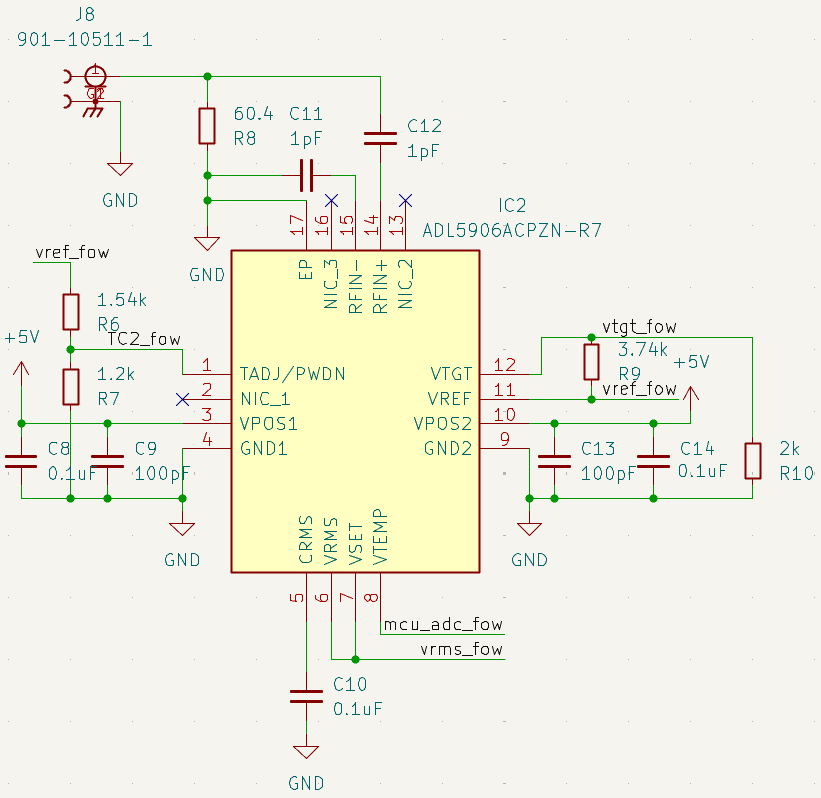
\includegraphics[width=0.5\textwidth]{pictures/fwd_powerdetector.png}\hspace{1cm}
    \caption{Jaudas noteikšanas integrālā shēma}
\end{figure}
Tika izveidota četru slāņu plate. Iespiedplates izstrādē liels uzsvars tika veikts uz pāris komponenšu izvēli, kondensatoru rezonanses frekvencei bija jābūt augstākai par mērāmo, celiņa platumam ieejā bija jābūt tādam, lai trakts būtu salāgots ar 50 ohm pretestību, SMA konektora kontaktlaukuma izmērs nedrīkstēja pārsniegt celiņa platumu, lai neveidotos signāla atstarojumi savienojuma vietā. Komponentes tika novietotas pēc iespējas tuvāk integrālajai shēmai, lai atbrīvotos no liekas parazītiskās induktivitātes. Trasējums veikts pēc datu lapas ieteikuma. 
\begin{figure}[H]
	\centering
    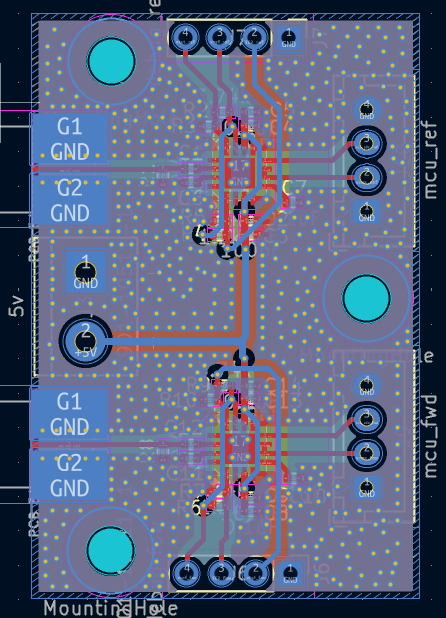
\includegraphics[width=0.6\textwidth]{pictures/board_powerdetector.png}\hspace{1cm}
    \caption{Jaudas noteikšanas iespiedplate}
\end{figure}

\subsection{Gala prototips}
1. pozīcijā ir HPA un uz viņa novietotie testa lauktranzistori, kas simulē jaudas pastiprinātājus. 2. pozīcijā ir līniju iezīmētie industriālie barošanas avoti. 3. pozīcijā ir monitorēšanas izstrādes plate. 4. pozīcijā ir mikrokontroliera plate. 5. pozīcijā ir RMS jaudas mērītājs. 6. pozīcijā ir pārveidotāju un barošanas avota vadības shēma. 7. pozīcija ir ieslēgšanas/izslēgšanas shēma ar strāvas mērīšanu. 
\begin{figure}[H]
	\centering
    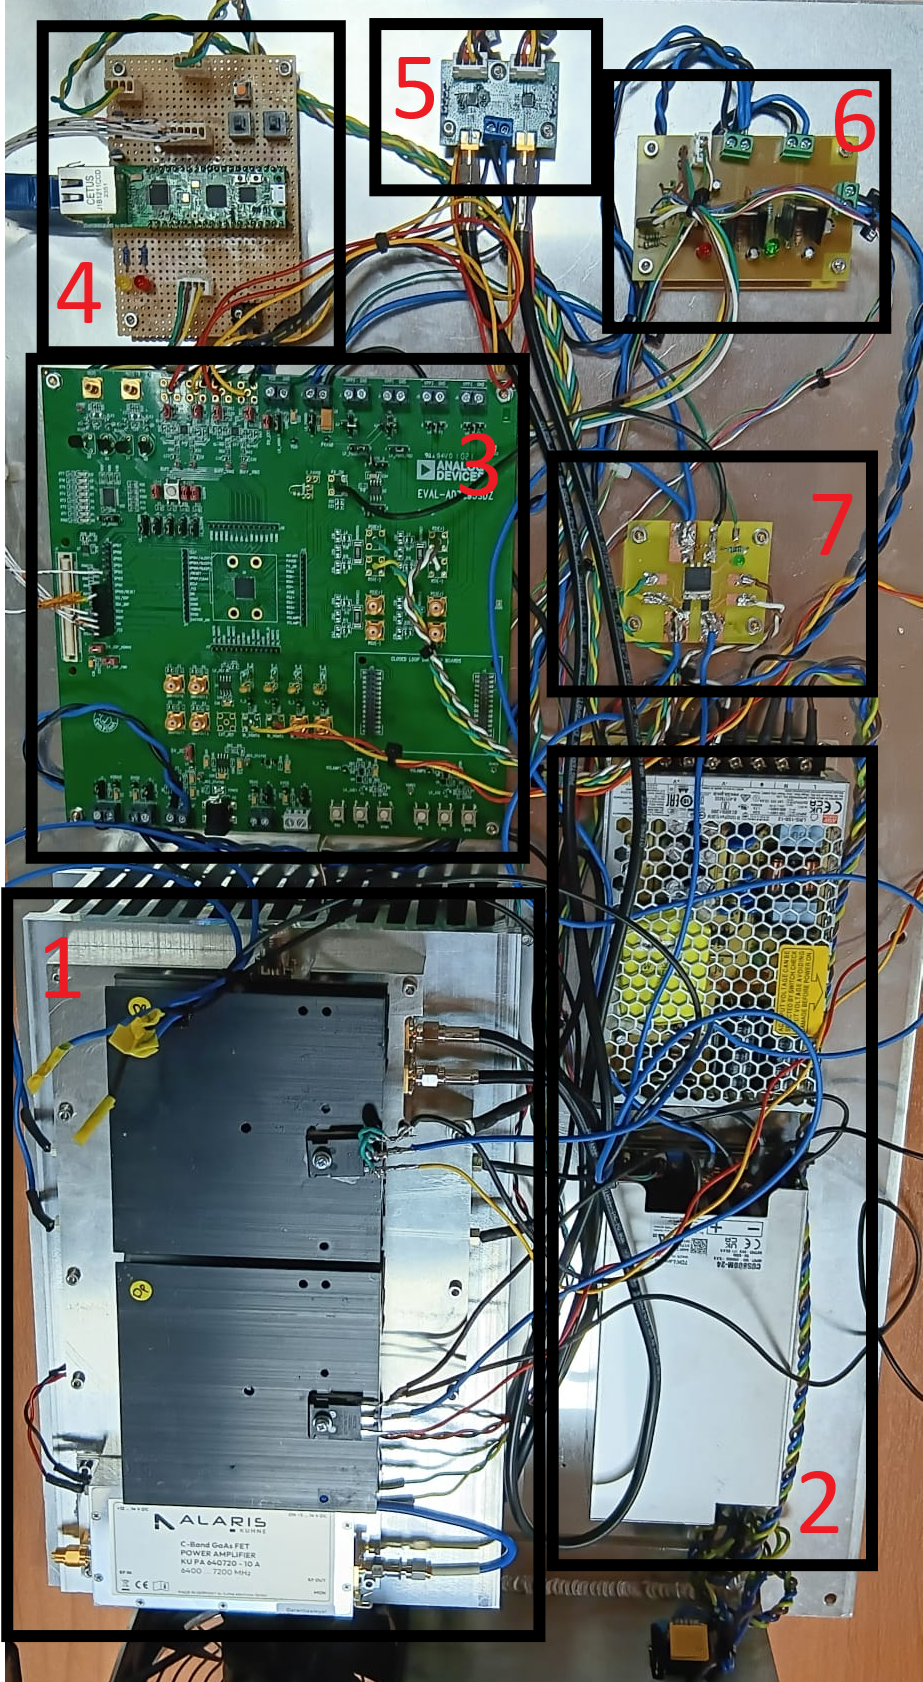
\includegraphics[width=0.9\textwidth]{pictures/finished.png}\hspace{1cm}
    \caption{Prototipa stends}
\end{figure}